\chapter{STRique Repeat Detection}
\label{cha:strique}

Expansions of short tandem repeats are genetic variants that have been implicated in several neuropsychiatric and other disorders, but their assessment remains challenging with current polymerase-based methods. Here we combine a CRISPR-Cas-based enrichment strategy for nanopore sequencing with an algorithm for raw signal analysis. Our method, termed \textit{STRique} for short tandem repeat identification, quantification and evaluation, integrates conventional sequence mapping of nanopore reads with raw signal alignment for the localization of repeat boundaries and a Hidden Markov Model based repeat counting mechanism. We demonstrate the precise quantification of repeat numbers in conjunction with the determination of CpG methylation states in the repeat expansion and in adjacent regions at the single-molecule level without amplification. Our method enables the study of previously inaccessible genomic regions and their epigenetic marks. \textit{STRique} is available at \textit{https://github.com/giesselmann/STRique}.

\begin{figure}[h]
    \centering
    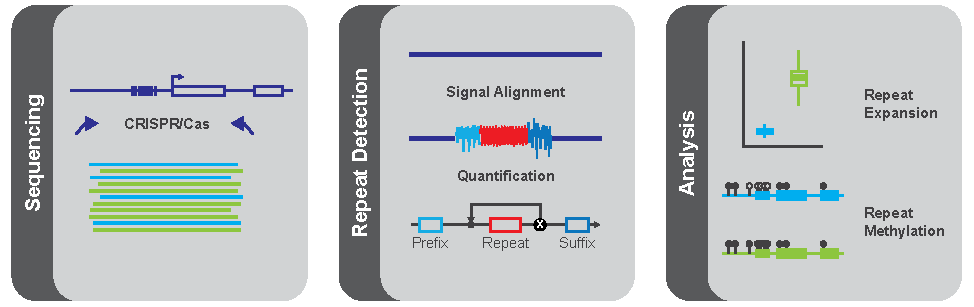
\includegraphics[width=1.0\textwidth]{figures/strique/GA.pdf}
    \label{fig:strique:ga}
\end{figure}

\textbf{Note:} This chapter is based on the publication P. Giesselmann et al. \textit{Analysis of short tandem repeat expansions and their methylation state with nanopore sequencing}, Nature Biotechnology, 2019 and contains text and figures from the original paper.

The chapter starts with a brief \textbf{background} in \ref{sec:strique:background}, followed by the evaluation of \textbf{sequenced based} repeat analysis in \ref{subsec:strique:seq_repeat_counts}. The development of an accurate \textbf{signal based} method is described in \ref{subsec:strique:sig_repeat_counts} and applied to patient samples with \textbf{c9orf72} and \textbf{FMR1} repeat expansions in \ref{subsec:strique:c9orf72}. Finally the DNA methylation detection on repeat and surrounding sequence is shown in \ref{sec:strique:modifications}.




\section{Background}
\label{sec:strique:background}

Short tandem repeats (STRs), also called microsatellite repeats, form the shortest class of tandem repeat elements in the genome. They consist of short nucleotide sequences (2 to 6 bp) concatenated without other sequence fragments in between. Distinguished by length, the next larger tandem repeat class, termed variable nucleotide tandem repeat (VNTR) or minisatellite repeat follows the same repeat pattern but from larger fragments (>6 bp). VNTRs are for instance used as genetic fingerprints in forensic crime investigations due to their highly variable lengths within populations \cite{Marwal2014}. Lastly alpha satellite repeats are a class of large {\textasciitilde171 bp} repeat elements structuring the centromeric regions of the human genome \cite{McNulty2018}.

The expansion of unstable genomic STRs is of particular interest as it causes more than 30 Mendelian human disorders \cite{Gatchel2005}. An extended GGGGCC-repeat $ [(G_{4}C_{2})_{n}] $ within the C9orf72 gene is the most frequent monogenic cause of Frontotemporal Dementia and Amyotrophic Lateral Sclerosis c9FTD/ALS \cite{Paulson2018}. Similarly, accumulation of a CGG motif in the FMR1 gene underlies the Fragile X Syndrome, and is currently one of the most common identifiable genetic causes of mental retardation and autism \cite{Verkerk1991}. In both repeat expansion disorders, recent evidence has suggested pronounced inter- and intraindividual repeat variability as well as focal changes in DNA methylation to modulate the disease phenotype \cite{Blitterswijk2013, Xi2013, Russ2015}. Repeat expansions of up to 100-150 repeats can still be analyzed with conventional PCR or short read based approaches. However in the clinical diagnostic setting, 'analog' southern blot analysis are still state of the art to estimate the repeat length. Requiring multiple days and suffering from decreased resolution for longer repeats, these workflows would benefit from a sequencing based approach, both time- and resolution-wise. For applications in the research sector, the combination of a high counting accuracy and the single-molecule resolution of nanopore sequencing provides unforeseen potential to gain better insights.

To get a first impression of the visibility of STRs in nanopore sequenced samples, we used the publicly available data from the human GM12878 cell line. The inspection revealed a characteristic pattern in raw nanopore read signals spanning the c9orf72 STR locus (Fig. \ref{fig:strique:signal}). 
To overcome current difficulties in characterizing expanded STRs we focused on three areas: i) optimization of nanopore sequencing and signal processing to capture STRs ii) development and implementation of a target enrichment strategy to increase efficiency and iii) integration of expansion measurements with CpG methylation at the single molecule level.
To enable a robust repeat analysis, we developed \textit{STRique}, a general-purpose signal processing algorithm for the exact quantification of STR numbers in raw nanopore signals.

\begin{figure}[h]
	\centering
	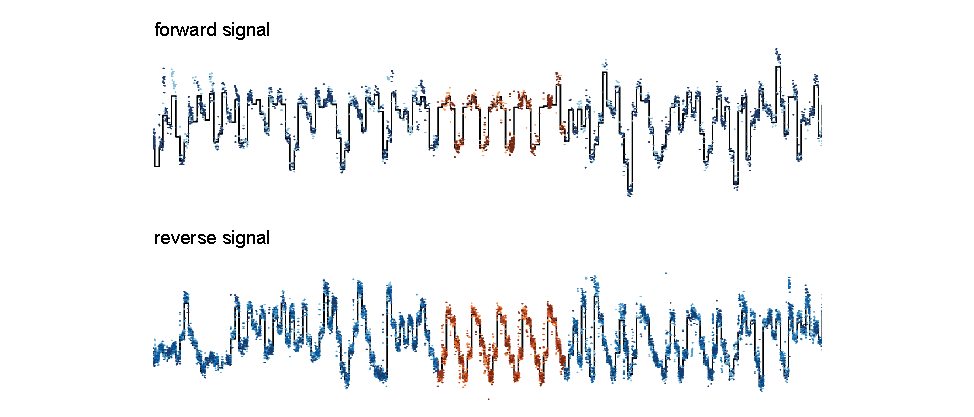
\includegraphics[width=1.0\textwidth]{figures/strique/signal.pdf}
	\captionsetup{format=plain}
	\caption[Nanopore raw signal of the C9orf72 STR in GM12878 cells]{Multi signal HMM alignment of publicly available raw traces from two forward and eight reverse strand reads from the GM12878 cell line shows matching signal pattern in all reads \cite{Jain2018}. Displayed are the current measurements as dots and the model signal as black line. Blue dots indicate current measurements identified as prefix or suffix sequence. Red dots indicate raw current measurements identified by \textit{STRique} as belonging to the C9orf72-$ (G_{4}C_{2})_{n} $-STR. \textit{STRique} detects in this case a $ (G_{4}C_{2})_{5} $-repeat.}
	\label{fig:strique:signal}
\end{figure}




\section{Repeat quantification}
\label{sec:strique:quantification}

Accurate counting of repeats with high resolution into even large expansion ranges serves as a first step during investigation of short tandem repeats. While a sequence based approach appears desirable due to a generally lower implementation complexity, the following sections illustrate the need for a signal based algorithm to exactly quantify the length of a short tandem repeat based on nanopore sequencing.

\subsection{Sequence based repeat detection}
\label{subsec:strique:seq_repeat_counts}

To first benchmark existing repeat expansion evaluation methods we constructed, verified and nanopore sequenced plasmids with several synthetic $ (G_{4}C_{2})_{n} $-repeat lengths \cite{Mizielinska2014}. As a baseline, we manually counted repeats for a subset of reads, exploiting the clear visibility of the repetitive signal pattern (Fig. \ref{fig:strique:signal}). Current (May 2019) production grade (\textit{guppy} v3.0.3, high accuracy model) software developed by Oxford Nanopore Technologies (ONT) was used to translate the raw signal into the respective nucleotide sequence. In order to determine the repeat length with existing methods we deployed a decoy-alignment approach (adapted from STRetch \cite{Dashnow2018}) and the \textit{RepeatHMM} \cite{Liu2017} package. For the alignment method we added decoy-chromosomes to the reference genome, each with a distinct repeat length in the range of 3 to 100 (e.g. chr\_9\_3 to chr\_9\_100). The quantification is based on the assumption, that individual reads with possibly different repeat lengths will align to the decoy-chromosome with the best matching length. Resolution and range of this approach are limited by the set of additional reference sequences.
\textit{RepeatHMM} was initially developed and tested for tri- (SCA3/ATXN3) and pentanucleotide (SCA10/ATXN10) repeat expansions and originally only reports an estimated repeat length distribution per target locus The software was forked\footnote{https://github.com/giesselmann/RepeatHMM, customized by Christian Rohrandt.} and modified to also work with the c9orf72 hexanucleotide repeat and to provide individual counts per read.

Both methods were evaluated on our synthetic repeat sequences (8, 32, 50, 56 and 76 $ G_{4}C_{2} $ repeats) and compared to the manual counted lengths. The analysis revealed, that current generation sequence based methods fail to satisfactorily resolve expanded STRs (Fig. \ref{fig:strique:count_seq_manual}).


\begin{figure}[h]
    \centering
    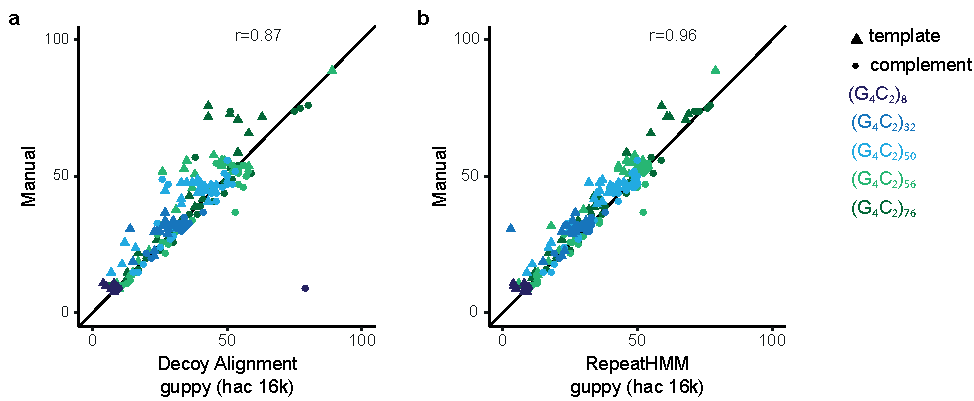
\includegraphics[width=1.0\textwidth]{figures/strique/count_seq_manual.pdf}
    \captionsetup{format=plain}
    \caption[Correlation and strand bias in STR analysis methods]{Manual counted set of plasmid reads on y-axis correlating with guppy basecalling and decoy alignment approach (\textbf{a}) and RepeatHMM (\textbf{b}) on x-axis. Only data points shown which could be evaluated with all three methods (n=15, 49, 45, 48, 47; Pearson correlation).}
    \label{fig:strique:count_seq_manual}
\end{figure}

Appreciating the constant development and improvement of neural network based basecalling software \cite{Wick2019} we systematically tested different versions and configurations. Specifically we deployed the previous state of the art software \textit{albacore} and the research and technology demonstration tool \textit{flappie} (both ONT). To keep memory requirements in a manageable range, these tools typically work on overlapping windows of the raw signal and combine these sub-sequences to the final output. For \textit{guppy} and \textit{albacore} the window size (default 1k and 10k respectively) is adjustable and we hypothesized that a larger basecalling window could improve the overall accuracy due to a larger context provided to the neural network. For \textit{guppy} we further tested two different models for fast and high accuracy predictions and computed correlations with the manually obtained counts in Fig. \ref{fig:strique:count_sequence_corr} a. 
Whereas the deprecated \textit{albacore} performed best in combination with the decoy alignment approach, sequences from \textit{guppy} with high accuracy model and increased window size resulted in the highest correlation with manual counts when evaluated with \textit{RepeatHMM} (Fig. \ref{fig:strique:count_sequence_corr} b). Further described and qualified in section \ref{subsec:strique:sig_repeat_counts}, our method \textit{STRique} outperforms any other approach on this level.

\begin{figure}[h]
	\centering
	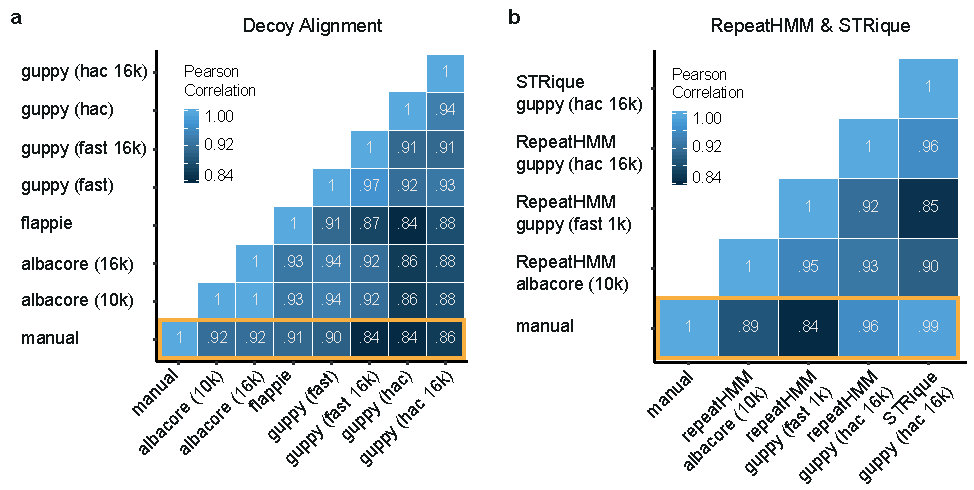
\includegraphics[width=1.0\textwidth]{figures/strique/count_sequence_corr.pdf}
	\captionsetup{format=plain}
	\caption[Correlation of sequence based STR detection methods]{\textbf{a}, Correlation of manual counted repeat lengths with sequence base methods. Decoy alignment against reference with 3-100 repeats with Albacore (window 10k and 16k), Guppy (fast and hac mode, 1k and 16k window size) and Flappie basecalling (n=204 reads). \textbf{b}, Correlation of manual count with RepeatHMM and \textit{STRique} results (n=204 reads).}
	\label{fig:strique:count_sequence_corr}
\end{figure}

To further assess the characteristics of existing workflows applied to larger repeat expansions, we next sequenced and analyzed the bacterial artificial chromosome (BAC) clone 239, generated from a c9FTD/ALS patient with an expected $ (G_{4}C_{2})_{800} $ repeat \cite{ORourke2015}. In absence of ground truth values per read we compare repeat counts across decoy alignment, \textit{RepeatHMM} and \textit{STRique} in Fig. \ref{fig:strique:count_bac}. Mostly masked by a band of comparatively short repeats, only \textit{STRique} is able to resolve a secondary peak at 800 repeats. More striking is the systematic strand bias observed in both sequence based methods resulting in generally more accurate counts for reads on the complement strand (GGGGCC repeat) compared to the template (GGCCCC repeat) strand.


\begin{figure}[h]
    \centering
    \includegraphics[width=1.0\textwidth]{figures/strique/count_bac.pdf}
    \captionsetup{format=plain}
    \caption[Strand bias in sequence based repeat counts]{Comparison of repeat counts from \textit{STRique}, decoy alignment based on guppy (high accuracy model, 16k window size) and repeatHMM based on guppy (high accuracy model, 16k window size) for BAC data. One dot (n=5004) per read passing all three approaches and colored by strand.}
    \label{fig:strique:count_bac}
\end{figure}

In conclusion, we find that nanopore sequencing in general is capable of reading through expanded short tandem repeats. However, existing sequenced based methods fail to accurately quantify repeat lengths beyond \textasciitilde32 hexanucleotide repeats. We further detect a strand and therefore sequence specific bias in the case of the c9orf72 $ G_{4}C_{2} $ repeat, requiring re-evaluation of methods per target and worst case per software and model version.




\subsection{Signal based repeat detection}
\label{subsec:strique:sig_repeat_counts}

For overcoming inaccuracies of sequence based methods our \textit{STRique} signal analysis software first identifies reads spanning a STR location by aligning the conventionally basecalled sequences to a reference \cite{Li2018}. Next, \textit{STRique} maps the upstream and downstream boundaries of the repeat within each read more precisely with a signal alignment algorithm and, as a third step, quantifies the number of any given STR sequence with a Hidden Markov Model (HMM, Fig. \ref{fig:strique:count_structure_plasmid}). 

\begin{figure}[h]
	\centering
	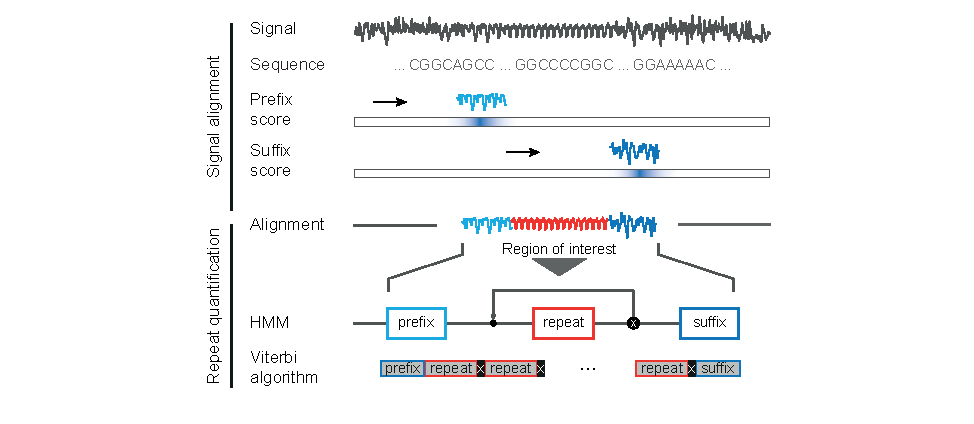
\includegraphics[width=1.0\textwidth]{figures/strique/count_structure_plasmid.pdf}
	\captionsetup{format=plain}
	\caption[\textit{STRique}: generic repeat detection pipeline on raw nanopore signals]{Repeat quantification enabled by raw signal alignment of flanking prefix and suffix regions and HMM-based count on the signal of interest.}
	\label{fig:strique:count_structure_plasmid}
\end{figure}

Raw signal normalization is a crucial first step prior to the quantification process. Due to the reduced complexity of the repetitive signal segment, the overall distribution of measurements is skewed compared to reads from regular genomic contexts. Both, mean and median centered normalization fail to project a signal containing a STR expansion and being affected by offset, scaling and drift over time into a uniform range. 
We therefore applied a min-max normalization by scaling the 0.025 and 0.975 quantiles of the raw signal to the respective values of the pore model.

With the normalized read and simulated signal fragments of the genomic sequence context around the STR, a signal alignment is used in order to locate prefix and suffix and to extract a region of interest. Within \textit{STRique}, we use the distance based semi-global alignment described in section \ref{sec:signal:alignment}. Depending on the sequence complexity of prefix and suffix, a 100 to 150 bp frame around the repeat appeared to be robust. Reads with overlapping or reversed order of prefix and suffix alignments are flagged and dropped in this step. Furthermore the alignment scores, equivalent to the sum of absolute differences between simulated and raw signal are part of the \textit{STRique} output and can be utilized to filter repeat counts in a post processing step.

Finally the actual repeat count is determined by a compound profile HMM composed of linear prefix and suffix modules, surrounding a single repeat instance with a feedback loop around (Fig. \ref{fig:strique:count_structure_plasmid}, section \ref{sec:signal:alignment}). The transition from repeat end to repeat begin enables the HMM to stay in the repeat associated states to model arbitrary long repeat expansions. The Viterbi algorithm assigns the most likely state from prefix, repeat and suffix to each observation of the normalized signal given the models states and transitions. The number of passes through the feedback transition is reported as the detected repeat count, the precise positions of prefix end and suffix begin are provided to enable masking of the repetitive signal fragment for downstream processing (cf. section \ref{subsec:strique:modifications_region}).

Aggregated \textit{STRique} repeat counts matched closely gel electrophoresis profiles (Bioanalyzer) from our synthetic repeat constructs and could be confirmed on the single molecule level by manually counting repeat patterns in raw signal traces (Fig. \ref{fig:strique:count_signal_corr}).

\begin{figure}[h]
	\centering
	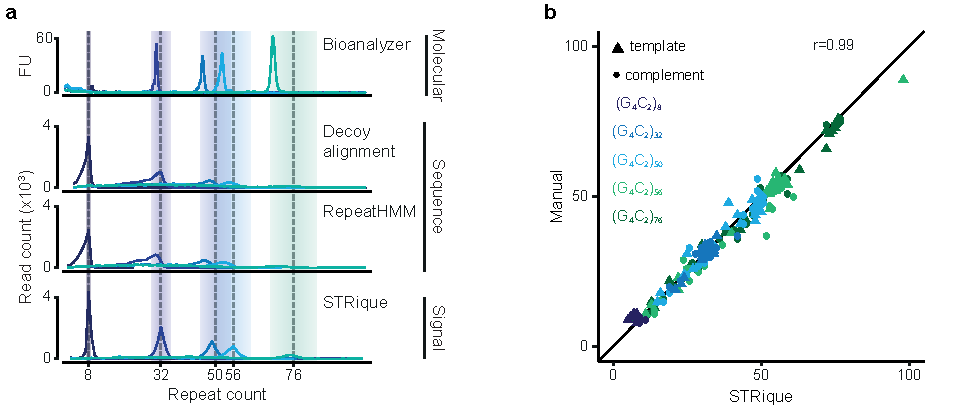
\includegraphics[width=1.0\textwidth]{figures/strique/count_signal_corr.pdf}
	\captionsetup{format=plain}
	\caption[Molecular, sequence and signal based STR evaluation]{\textbf{a}, Bioanalyzer electropherogram, decoy alignment, \textit{RepeatHMM} and \textit{STRique} counts of synthetic $ (G_{4}C_{2})_{n} $ repeats. \textbf{b}, Manual counted set of plasmid reads on y-axis correlating with \textit{STRique} raw signal pipeline on x-axis. Only data points shown which could also be evaluated with methods in Fig. \ref{fig:strique:count_seq_manual} (n=15, 49, 45, 48, 47; Pearson correlation).}
	\label{fig:strique:count_signal_corr}
\end{figure}

\textit{STRique} is written in python3 with a C++ extension for the signal alignment, supports multiprocessing and is automatically build and tested using Travis-CI. \textit{STRique} is deployed either as a python3 virtual environment or as a standalone Docker container.




\subsection{Repeat expansion in C9orf72 and FMR1}
\label{subsec:strique:c9orf72}

The nanopore sequencing of repeats integrated into plasmid or BAC backbones typically yields thousands of reads containing the expanded repeat. For the application in disease contexts, the sequencing of DNA from e.g. patient-derived induced pluripotent stem cell lines is favored, as it for instance preserves the epigenetic landscape around the repeat. However, a straightforward whole genome sequencing would only yield few reads covering the repeat of interest. From e.g. 30 Gbp throughput, equivalent to 10 fold genome wide coverage, on average only 10 reads would be expected to cover any target repeat. For the monoallelic expansions in the C9orf72 and FMR1 genes, only half of those would be informative to infer the repeat length.

To increase the amount of reads covering any repeat expansion of interest, we therefore set up a CRISPR-Cas9 target enrichment strategy. Briefly, during library preparation, the method cuts the DNA on defined guide sequences next to the target locus. Following on a dephosphorylation step during fragmentation, only the Cas9 cleaved and therefore phosphorylated ends are capable to ligate the ONT sequencing adapter. Hence only fragments starting on definable guide sequences are sequenced on the nanopore flow cell.
We applied enrichment and quantification to one C9orf72 repeat expansion patient derived stem cell line (24/5\#2) and two patient derived cell lines (SC105-iPS6/iPS7) from another patient with a FMR1 repeat expansion (Fig. \ref{fig:strique:count_patients}).


\begin{figure}[h]
    \centering
    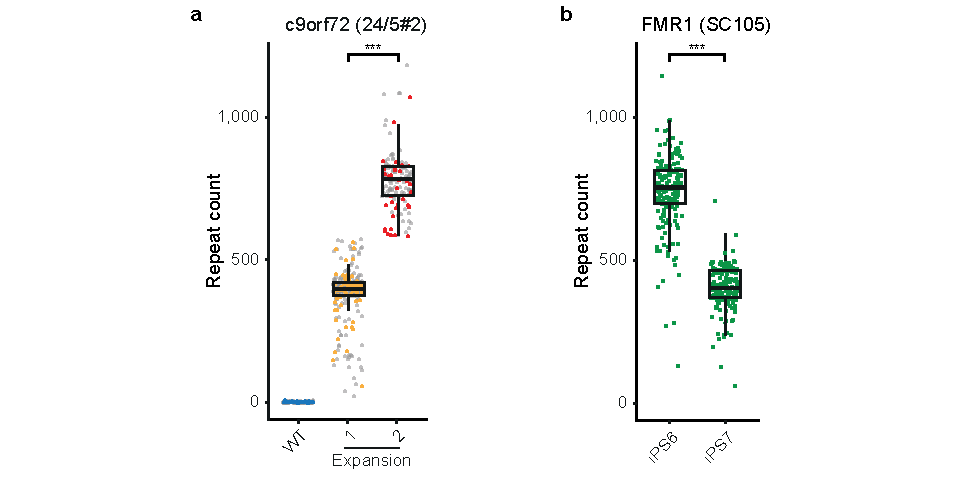
\includegraphics[width=1.0\textwidth]{figures/strique/count_patient_samples.pdf}
    \captionsetup{format=plain}
    \caption[Repeat quantification in C9orf72 and FMR1 patients]{\textbf{a}, Repeat quantification of sample 24/5\#2 at the C9orf72 locus, revealing two distinct repeat bands of \textasciitilde450 and \textasciitilde750 $ G_{4}C_{2} $ repeats (n = 1,810, 738 and 363 evaluated reads with a difference in repeat length of 392 (95\% confidence interval (CI): 383 to 400), $ P < 2.2 \cdot 10^{-16} $). Colored points indicate reads used in Fig. \ref{fig:strique:methylation_c9orf72_region}b. WT, wild type. \textbf{b}, Repeat quantification of the SC105iPS6 and SC105iPS7 samples at the FMR1 locus (n = 174 and 168 evaluated reads with a difference in repeat length of -343 (95\% CI: -361 to -325), $ P < 2.2 \cdot 10^{-16} $). P values in a and b were obtained by a two-sided Wilcoxon rank-sum test; $ ***P < 0.001 $. Data are presented as boxplots (centerline, median; box limits, first and third quartiles; whiskers, 1.5x interquartile range).}
    \label{fig:strique:count_patients}
\end{figure}


In the C9orf72 case, the analysis revealed two distinct repeat expansion bands next to the wild type allele with \textasciitilde450 and \textasciitilde750 $ G_{4}C_{2} $ repeats respectively. Even though derived from the same male patient, the two FMR1 samples showed different repeat lengths with a difference of 343 CGG repeats. During development and improvement of the enrichment protocol, both samples were sequenced multiple times on the MinION and PromethION platform. Nonetheless, the two repeat expansion cluster are already detectable from the output of a single MinION sequencing run with up to thousand reads on target (Fig. \ref{fig:strique:count_experiments}, FAK67994)


\begin{figure}[h]
    \centering
    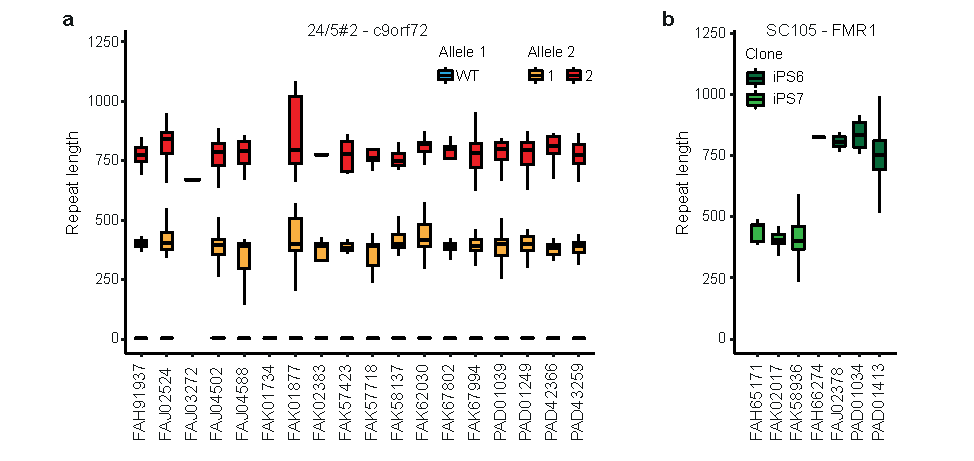
\includegraphics[width=1.0\textwidth]{figures/strique/count_experiments.pdf}
    \captionsetup{format=plain}
    \caption[Repeat count cluster stability over experiments]{\textbf{a}, C9orf72 target enrichment flow cells for patient 24/5\#2 \textbf{b}, FMR1 enrichment flow cells of SC105iPS6/iPS7. (FA*: MinION, PAD*: PromethION, number of reads per boxplot are in Supplementary Tables \ref{tab:strique:Cas12} and \ref{tab:strique:Cas9}). Data presented as boxplots (centerline, median; box limits, first and third quartiles; whiskers, 1.5x interquartile range; outliers not shown)}
    \label{fig:strique:count_experiments}
\end{figure}

In summary we show, that even heterogeneous expansion distributions of any short tandem repeat can be sequenced and quantified from a single MinION flow cell. In comparison to established southern blotting, our approach increases the accuracy and adds the resolution of single molecule counts. In combination with target enrichment, the workflow could be deployed to provide same-day analysis in a clinical environment.




\section{Methylation detection}
\label{sec:strique:modifications}

The epigenetic modification of C9orf72 and FMR1 loci have been correlated with STR expansion status and patient characteristics in both disorders, however without quantification at the single molecule level so far \cite{Russ2015, Hornstra1993}. Additionally, in c9FTD/ALS patients pervasive CpG methylation of the $ G_{4}C_{2} $-repeat itself has been reported \cite{Xi2015}. Assessed with a strictly qualitative assay, the expanded STR itself was reported to be methylated in the majority of cases examined. A similar observation has been directly implicated in the pathogenesis of FXS, where a CGG repeat expansion at the FMR1-locus beyond a threshold of > 200 repeats leads in most cases to the silencing of the entire FMR1-gene through CpG-methylation \cite{Lyons2015}. Exploiting the visibility of 5-methylcytosine in nanopore sequencing, we extend \textit{STRique} in the following sections to integrate repeat length and DNA methylation status on the same molecule.


\subsection{Region methylation detection}
\label{subsec:strique:modifications_region}

Nanopore reads spanning an expanded STR location can be aligned to a reference genome using standard tools like \textit{minimap2} \cite{Li2018}. Though, due to the potentially large insertion, the reads are commonly soft-clipped from one side up to the STR, mapping either prefix or suffix. While this is sufficient to identify reads spanning the target locus during quantification of the repeat length, it does not allow the direct readout of the DNA methylation status on both sides of the repeat. We therefore use the signal level information of the exact position of the STR within the read from the previous quantification and provide a script (fast5Masker.py) to trim the STR signal fragment from each read (cf. red signal segment in Fig \ref{fig:strique:count_structure_plasmid}). The resulting traces are stored as regular fast5 files and can be processed with any standard pipeline. The manipulation of the raw signal leads to minor basecalling errors directly adjacent to the STR, but enables the mapping of both flanking sequences to the reference genome.

Hereafter we integrated single read CpG methylation analysis of regions adjacent to the c9orf72 STR using \textit{nanopolish} \cite{Simpson2017} with our \textit{STRique} results (Fig. \ref{fig:strique:methylation_c9orf72_region} a). We found that in the 24/5\#2 line all reads with STR expansions > 750 repeats showed a significantly increased methylation level at the promoter CpG island. In contrast all wild type reads and those with \textasciitilde450 repeats were not or only partially methylated (Two sided Wilcoxon rank sum test p < 0.001, Fig. \ref{fig:strique:methylation_c9orf72_region} b).

\begin{figure}[h]
    \centering
    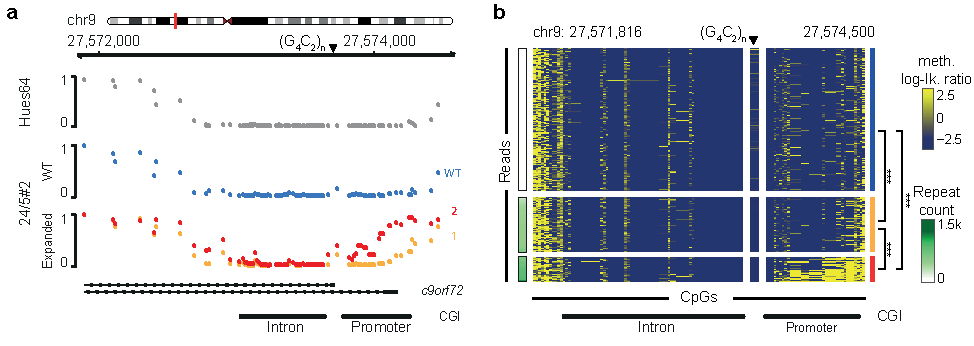
\includegraphics[width=1.0\textwidth]{figures/strique/methylation_c9orf72_region.pdf}
    \captionsetup{format=plain}
    \caption[Methylation state analyses at the single-read level]{\textbf{a}, C9orf72 methylation status in HUES64 as measured by whole-genome bisulfite sequencing. The wild-type (blue) allele and expanded (ex; orange) alleles (with 450 and 750 $ (G_{4}C_{2})_{n} $ repeats (red), respectively) are shown for patient 24/5\#2, as measured by nanopore sequencing. \textbf{b}, Single read nanopore methylation of C9orf72 covering reads from the minus strand (n = 259, 100 and 43 rows per block) sorted by detected repeat length (rows, single read; columns, single CpGs). CpGs with logP ratio $> 2.5$ are considered methylated, while those with logP ratio $< -2.5$ are considered unmethylated. The median methylation difference (95\% CI) and P value (determined by two-sided Wilcoxon rank-sum test on mean promoter CGI methylation) for comparisons were as follows: $ WT-ex450: 3.9 \cdot 10^{-5} (4.8 \cdot 10^{-6} to 3.4 \cdot 10^{-2}), P = 5.3 \cdot 10^{-9}; WT-ex750: 0.56 (0.46-0.64), P < 2.2 \cdot 10^{-16}; ex450-ex750: 0.53 (0.40-0.64), P < 2.2 \cdot 10^{-16}; ***P < 0.001. $ }
    \label{fig:strique:methylation_c9orf72_region}
\end{figure}

Masking segments of the raw nanopore signal is a considerable change of the original measurement. We therefore validated the region methylation detection approach on our previously introduced BAC data. Amplified in bacteria, the artificial chromosome is free of CpG methylation but contains a larger sequence window around the repeat on chromosome 9 making it comparable to the patient data. Applying the same workflow of repeat quantification, masking and nanopolish methylation detection, we find no 5-methylcytosine signal in any of the BAC reads independent of the repeat length (Fig. \ref{fig:strique:methylation_bac_region} a,b). Comparing the mean methylation rates between patient 24/5\#2 and BAC, we find no evidence for a difference on the intron CGI, but significant level differences in particular for the \textasciitilde750 repeat cluster on the promoter CGI.

In summary, the STR detection on signal level facilitates the reconstruction of wild type like reads from large STR expansions, enabling execution of established workflows.

\begin{figure}[h]
    \centering
    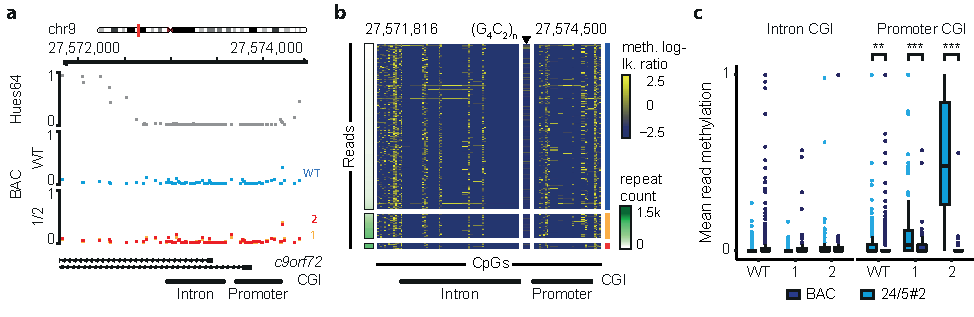
\includegraphics[width=1.0\textwidth]{figures/strique/methylation_bac_region.pdf}
    \captionsetup{format=plain}
    \caption[Nanopore single read methylation in BAC data]{\textbf{a}, Methylation status of c9orf72 region in BAC data for repeats < 200 (WT), 200-750 (Cluster1,orange) and > 750 (Cluster2,red) and control (HUES64, WGBS) \textbf{b}, Single read methylation on a sample of 500 BAC minus strand reads sorted by repeat count (row split 200 and 750 repeats, n=423,63,14). \textbf{c}, Difference in mean CGI methylation of intron and promoter per read on minus strand. Reads binned by detected repeat length for BAC (n=2066 WT; 315 Cluster1; 72 Cluster2) and patient 24/5\#2 (n=925 WT; 362 Cluster1; 153 Cluster2). Two sided Wilcoxon rank sum test, corrected for multiple testing (Holm), q-vals: * 0.05 - 0.01; ** 0.01 - 0.001; *** < 0.001. Median methylation differences between promoter CGI [95\%CI] for WT $-2.3e^{-5} [CI: -5.6e^{-6}:-1.5e^{-5}, q=7.4e^{-3}] $ and Cluster1 $ -0.01 [CI: -7.1e^{-5}:-3.4e^{-2}, q=1.4e^{-17}] $ and Cluster2 $ -0.46 [CI: -0.58:-0.37, q=1.0e^{-26}] $.}
    \label{fig:strique:methylation_bac_region}
\end{figure}




\subsection{Repeat methylation detection}
\label{subsec:strique:modifications_repeat}


Due to the intrinsic heterogeneity in STR length, reference genome based methods such as \textit{nanopolish} cannot be used to determine CpG methylation on the repeat expansion itself. To detect 5mC modifications on STRs, we extended \textit{STRique} by employing a parallel HMM with unmodified- and 5mC-paths. Taking the expected signal levels for native and 5mC modified DNA from nanopolish, the profile-HMM block modeling the repeat is replaced by two parallel blocks, allowing the full HMM to switch between methylated and native path during each repeat iteration.
This single read analysis returns a methylation state for each tandem repeat, which then can be summarized into the mean repeat methylation level over the whole repetitive sequence.

When applying the methylation-aware \textit{STRique}, all expanded FMR1-STRs in nanopore reads from patient SC105 are found to be highly methylated (Fig. \ref{fig:strique:methylation_repeat} a), consistent with previous analyses \cite{Hornstra1993}. We next evaluated this approach on plasmids containing n=76 synthetic $ G_{4}C_{2} $ and n=99 CGG-repeats (Addgene, \#63089), which were covalently modified with the methyltransferase M.SssI (Fig. \ref{fig:strique:methylation_repeat} b,c). In addition we tested the algorithm on $ (G_{4}C_{2})_{n} $-containing reads from patient-derived DNA, which had been modified with M.SssI in vitro. In summary, we found that \textit{STRique} can determine the repeat CpG methylation state correctly in all positive and negative controls evaluated.
Surprisingly though, all reads covering the C9orf72-STR from our patient-derived samples showed little to no CpG-methylation, independently of the repeat expansion length or methylation status of the promoter CGI (Fig. \ref{fig:strique:methylation_c9orf72_region} b, center column).




\begin{figure}[h]
    \centering
    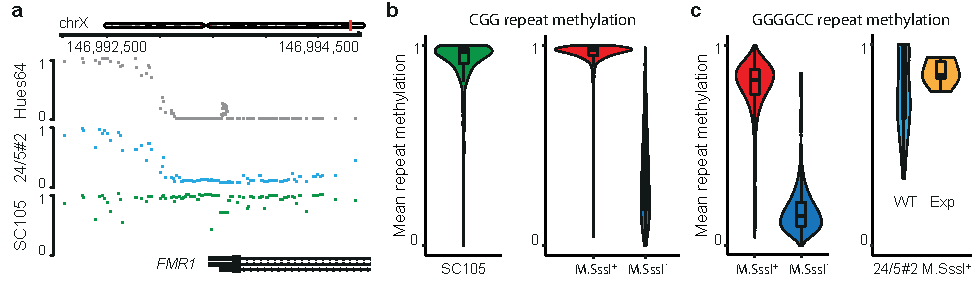
\includegraphics[width=1.0\textwidth]{figures/strique/methylation_repeat.pdf}
    \captionsetup{format=plain}
    \caption[Region and repeat methylation detection]{\textbf{a}, FMR1 region methylation in SC105iPS6/iPS7 compared to HUES64 WGBS and patient sample 24/5\#2. \textbf{b}, CGG mean repeat methylation status detected by \textit{STRique} for SC105 (n=197) and synthetic plasmid control with 99 repeats treated with $ M.SssI^{+/-} $ (5mC level on minus strand, n=1232 $ M.SssI^{+} $; n=11991 $ M.SssI^{-} $). \textbf{c}, GGGGCC repeat methylation status for plasmid control with 76 repeats treated with $ M.SssI^{+/-} $ (n=2939 $ M.SssI^{+} $; n=31280 $ M.SssI^{-} $) and patient sample 24/5\#2 treated with $ M.SssI^{+} $ (5mC level on minus strand, n=52 WT and n=6 Cluster1). Data in (b-c) presented as violin plots with overlayed boxplots (centerline, median; box limits, first and third quartiles; whiskers, 1.5x interquartile range; outliers not shown).}
    \label{fig:strique:methylation_repeat}
\end{figure}




\section{Summary}
\label{sec:strique:summary}

Our results demonstrate the precise and multi-layered molecular characterization of pathological short tandem repeat expansions. The CRISPR/Cas-nuclease-target enrichment and \textit{STRique} can be rapidly adapted to any other genomic region of interest, ensuring broad applicability to overcome challenges associated with the single molecule analysis. This allows for immediate integration of genetic and epigenetic signals associated with unstable repeat expansions or any other as of yet unsequenceable genomic regions in human health and disease. This type of analysis improves diagnostic workflows in regard to accuracy and resolution of unstable repeat expansion while enabling efforts to gain mechanistic insights into effects on differentiation, aging and future therapeutic agents that modify DNA methylation.


